En este capítulo se mostrará todo el proceso que se ha seguido para el desarrollo del prototipo
de apoyo a la toma de decisiones en esgrima. Para ello se ha seguido la dinámica \textit{Agile Inception}
para el inicio del proyecto y después utilizando el desarrollo iterativo e incremental para
las primeras versiones.

Para la resolución del proyecto han sido necesarias cinco iteraciones para cubrir
los objetivos propuestos en el Capítulo 1 (Ver figura 5.1).

\begin{figure}[htb]
  \centering
    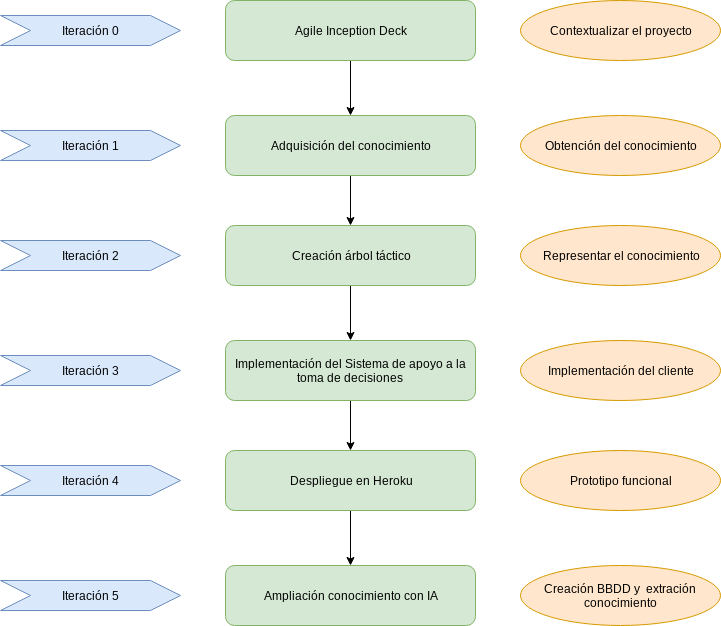
\includegraphics[width=0.8\linewidth]{Iteraciones}
  \caption[Desarrollo SE]{Desarrollo SE}
  \label{fig:Desarrollo Sistema Experto}
\end{figure}

\section{Agile Inception Deck}

Puesto que el proyecto junta dos disciplinas muy diferentes como son informática y esgrima,
es imprescindible que todas las partes del proyecto que están involucradas y remen en la misma
dirección. Para ello se utilizará la metodología \textit{Agile Inception Deck}

\subsection{¿Por qué estamos aquí?}
La necesidad de un apoyo a la toma de decisiones en una competición de esgrima es innegable.
En la élite los tiradores tendrán entrenadores dedicados a ellos con estudios previos de rivales.
Pero en niveles inferiores no se dará el caso, por lo que el desarrollo de un sistema de
apoyo a la toma de decisiones será de gran utilidad para la comunidad de esgrima en las
competiciones.

Además, en las salas de esgrima muchas veces no se dispone del tiempo suficiente para que un
entrenador pueda transmitir su conocimiento a los alumnos, o no hay un entrenador como tal
puesto que algunos clubes han empezado siendo un grupo de amigos que han practicado el deporte
y querían que hubiera un club en su ciudad, sin tener estos muchos conocimientos. Para estos
casos en los que se tienen dudas sobre que hacer en ciertas situaciones, este sistema
dará una respuesta teórica para aclarar su visión.

Volviendo al mundo de la competición, también servirá a aquellos competidores que quieran
averiguar si la elección que hicieron fue la correcta. Después de un torneo son muchos
los que piensan que ha pasado, pudiendo usar la herramienta para saber si fue muy
disparatada la elección.

\subsection{El \textit{Elevator pitch}}
Aquí se tratará de explicar la finalidad del proyecto con la mayor brevedad posible. Para ello
se elaboró la siguiente definición del prototipo:

Sistema de apoyo a la toma de decisión en un asalto de esgrima haciendo uso del
conocimiento extraído de expertos y análisis de datos. Para llegar a dicho sistema
se utilizarán técnicas de Ingeniería del conocimiento junto a técnicas de Inteligencia
Artificial.

\subsection{Diseñar una caja para el producto}
El prototipo del proyecto surge de la necesidad de apoyar (o cubrir en caso de que no exista)
la figura de entrenador en un asalto de esgrima para el arma de espada. Suponiendo que el
producto final cubra las tres armas la imagen idónea para el producto sería:

\begin{itemize}
  \item Ayudar a los competidores y entrenadores de esgrima a poder plantear una táctica antes
    del primer asalto y cambiarla en los descansos teniendo un sistema
    que le de opciones según las características de los tiradores.
  \item Ayudar a los practicantes de esgrima para que puedan ampliar y afianzar conocimientos
    sobre posibles situaciones sin tener que exponerse a ellas.
  \item Ayudar a la pérdida de practicantes de este deporte en las primeras competiciones haciendo
    que la curva de aprendizaje sea menor.
\end{itemize}

El prototipo limita la imagen idónea a un arma, pero la finalidad es la misma para el resto.
\subsection{Lista de los no}
Dado que es un prototipo se han definido una serie de limitaciones para disminuir la duración
del proyecto:
\begin{itemize}
  \item Alcance del prototipo:
    \begin{itemize}
      \item El prototipo será diseñado únicamente para la categoría de espada.
      \item El prototipo contemplará las acciones básicas e intermedias de espada.
      \item El prototipo contemplará las combinaciones básicas de espada.
      \item El prototipo contará con dos versiones. Una de ellas será de uso rápido
        (preguntas y respuestas sencillas), mientras que la otra será mas detallada
        en la introducción de sus entradas y en las salidas que de.
    \end{itemize}
  \item Fuera del alcance:
    \begin{itemize}
      \item Sistema para las categorías de florete y sable.
      \item No estarán contempladas todas las acciones posibles dentro del prototipo.
      \item No estarán contempladas todas las combinaciones posibles dentro del prototipo.
    \end{itemize}
\end{itemize}

\subsection{Conoce a tus vecinos}
En esta sección hablaremos sobre las personas involucradas en el proyecto. Los componentes
del proyecto son los siguientes:
\begin{itemize}
  \item Autor del proyecto:
    \begin{itemize}
      \item Gregorio Baldomero Patiño Esteo
    \end{itemize}
  \item Director del proyecto:
    \begin{itemize}
      \item Dr. José Ángel Olivas Varela.
    \end{itemize}
  \item Expertos implicados:
    \begin{itemize}
      \item Juan Lomas Rayego
    \end{itemize}
  \item Clubs implicados:
    \begin{itemize}
      \item Espadas de Calatrava (Ciudad Real)
    \end{itemize}
\end{itemize}

\subsection{Muestra la solución}
En este apartado se muestra un resumen de la arquitectura del proyecto a alto nivel
(Ver figura 5.2) y las herramientas empleadas para el desarrollo del mismo.

\begin{figure}[htb]
  \centering
    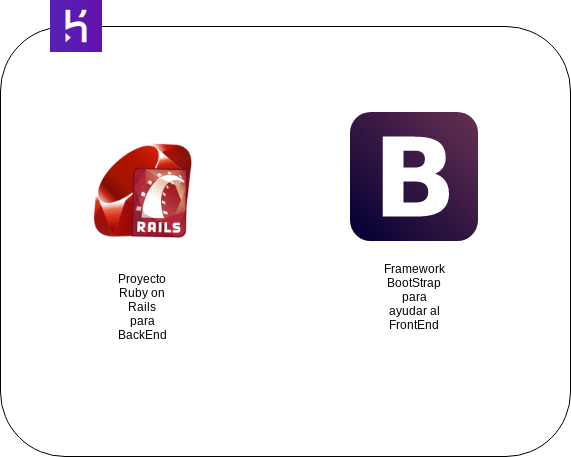
\includegraphics[width=0.4\linewidth]{Arquitectura}
  \caption[Desarrollo SE]{Desarrollo SE}
  \label{fig:Desarrollo Sistema Experto}
\end{figure}


Para llevar a cabo el proyecto se han empleado las siguientes herramientas:
\begin{itemize}
  \item \textbf{Python:} como lenguaje de programación para la extracción de datos e implementación
    de algoritmos.
  \item \textbf{Clips:} como lenguaje para la creación de reglas del primer prototipo
  \item \textbf{Latex:} lenguaje para la documentación del proyecto. La plantilla utilizada
    ha sido desarrollada por el profesor David Villa Alises.
  \item \textbf{Ruby on Rails:} como lenguaje y framework para la aplicación web.
  \item \textbf{Heroku:} para despliegue de entornos en producción.
  \item \textbf{Numpy:} librería usada para el tratamiento de datos y creación de BBDD.
  \item \textbf{BeatifulSoup:} librería usada para la extracción de datos.
  \item \textbf{SciKit:} librería usada para el análisis de datos.
  \item \textbf{Vim:} Editor utilizado para RoR y LaTeX.
  \item \textbf{TexStudio:} IDE utilizado para compilar documentos en LaTeX.
  \item \textbf{Spyder:} IDE utilizado para compilación de Python.
  \item \textbf{Anaconda:} Framework utilizado para instalar los entornos de Python.
  \item \textbf{Github:} aplicación web utilizada para la creación y gestión de repositorios.
    Además también ha sido usada para tener un tablon kanvan.
  \item \textbf{Firefox:} navegador usado para la extración de datos.
  \item \textbf{Draw.io:} aplicación web utilizada para la creación de gráficos, prototipos
    y diagramas.
\end{itemize}

\subsection{¿Qué nos quita el sueño por las noches?}
El principal problema que nos podemos encontrar a la hora de realizar el proyecto
es la situacionalidad de los casos a analizar. Puesto que aunque teóricamente
sea correcto una acción frente a otra, dependerá de ambos tiradores que esta
sea la correcta. Es por esto que se intentará hacer un sistema lo mas completo posible.

\subsection{Tamaño del proyecto}
Puesto que el sistema ha de ser bastante completo para tener una alta fiabilidad
será complicado dar una aproximación precisa. Es por esto que se hará una estimación,
teniendo muy presente que son estimaciones y puede variar. La estimación se dará en
tiempo dedicado sin indicar fechas dada la disponibilidad de los recursos. La linea
temporal del proyecto se puede ver en la figura 5.3 expuesta a continuación.

\begin{figure}[htb]
  \centering
    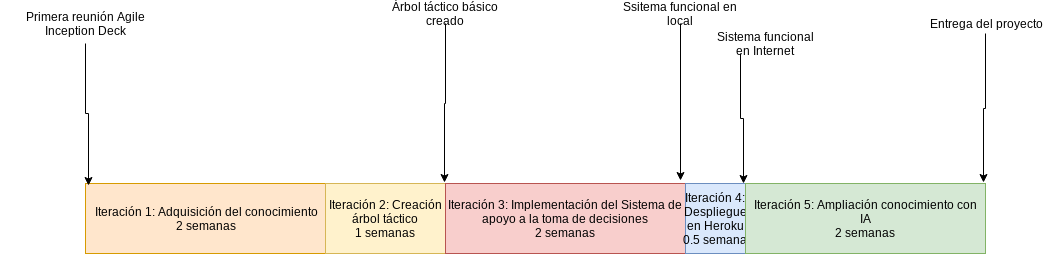
\includegraphics[width=0.95\linewidth]{LineaTemporal}
  \caption[Desarrollo SE]{Desarrollo SE}
  \label{fig:Desarrollo Sistema Experto}
\end{figure}

\subsection{Muestra con claridad lo que se va a dar}
Los objetivos a cumplir son los siguientes:

\begin{itemize}
  \item Establecimiento del dominio del proyecto.
  \item Adquisición del conocimiento.
  \item Representación del conocimiento con cliente Ruby on Rails para
    un fácil uso e interacción con el prototipo.
  \item Despliegue de la infraestructura del servicio en Heroku.
\end{itemize}

\subsection{Muestra lo que va a conllevar}
El análisis de costes del proyecto se llevará a cabo basándose a la planificación que se
puede ver en el punto 8 (ver Figura 5.3).
Los costes del proyecto se pueden dividir principalmente en dos tipos: personal e infraestructura.

El primer tipo, personal, dependerá del rol que se tome, puesto que dependiendo de este
el coste a la hora será mayor. El primer rol que tendremos será el de desarrollador, el
cual está estimado en 16€/h. Por otro lado tendremos el rol de experto, cuyo valor está estimado
en 30€/h. En la tabla 5.1 se puede ver el coste de cada iteración, por rol y por horas.
Además se podrá ver el coste total.

\begin{table}[]
  \centering
  \caption{Horas del proyecto}
  \label{tab:Horas del proyecto}
  \begin{tabular}{|l|l|l|}
    \hline
    Etapas & Horas dedicadas por autor & Hora dedicadas por Experto \\ \hline
    Iteración 0 & 4h & 4h \\ \hline
    Iteración 1 & 76h & 20h \\ \hline
    Iteración 2 & 40h & 5h \\ \hline
    Iteración 3 & 80h & 10h \\ \hline
    Iteración 4 & 20h & 0h \\ \hline
    Iteración 5 & 80h & 5h \\ \hline
    Total & 300 & 44 \\ \hline
  \end{tabular}
\end{table}

Por otro lado los costes de infraestructura han sido reducidos a cero. Puesto que no se
busca lucrarse con el uso de herramienta, si no que sea útil para el resto se han buscado
alternativas para reducir el coste disminuyendo en rendimiento de estas. Se ha optado
por Heroku puesto que ofrece un plan totalmente gratuito a pesar de sus bajos recursos.
Estos serán ampliables según las necesidades que se tengan.

Por lo que el coste total del proyecto puede verse en la tabla 5.2

\begin{table}[]
  \centering
  \caption{Costes del proyecto}
  \label{tab:Costes del proyecto}
  \begin{tabular}{|c|c|l|l|}
    \hline
    Concepto & Desglose & Horas & Coste \\ \hline
    \multirow{2}{*}{Personal} & Autor del proyecto & 300h & 4800€ \\ \cline{2-4}
    & Experto & 44h & 1320€ \\ \hline
    Infraestructura & Heroku proyect & - & 0€ \\ \hline
    Total & \multicolumn{3}{c|}{6120€} \\ \hline
  \end{tabular}
\end{table}
